\documentclass[a4paper]{article}
\usepackage[utf8]{inputenc}
\usepackage{caption}
\usepackage{subcaption}
\usepackage[spanish]{babel}
\usepackage{graphicx}
\usepackage{xcolor}
\usepackage{amsmath}
\usepackage{hyperref}
\usepackage{todonotes}
\usepackage{biblatex}

\newcommand\imgScale {0.6}

\addbibresource{biblio.bib}

\title{Proyecto visión avanzada}
\author{Raúl Candela Arias \\ Francisco Morillas Espejo}
\date{Abril 2021}

\begin{document}

\maketitle

\section{Introducción}

El objetivo de este proyecto es el entrenamiento de redes convolucionales para realizar \textbf{segmentación semántica} de imágenes para detectar hasta \todo[fancyline]{revisar numero de clases}3 clases diferentes.
\newline

La segmentación semántica consiste en, dada una imagen, identificar a que clase de elemento corresponde cada píxel de esta.
Para ello, se crea una máscara de las mismas dimensiones que la imagen de entrada donde previamente se han coloreado las distintas clases (objetos) que se desean identificar (figura~\ref{fig:semanticSeg}).
\newline

La imagen original y la máscara se relacionan tal que, sea $A$ la imagen de entrada y $M$ la máscara, para cada píxel de la imagen $A_{i,j}$ tenemos que $M_{i,j} = c(A,i,j)$, donde $c$ es una función que indica a que clase pertenece el píxel ubicado en la imagen $A$ en la posición $i,j$.
\begin{figure}[htbp]
    \centering
    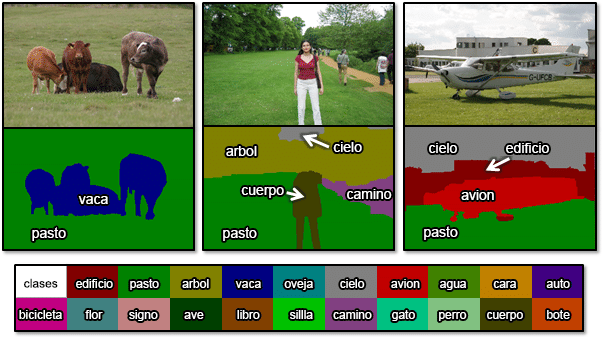
\includegraphics[scale=\imgScale]{img/EjSegSem.png}
    \caption{\small Ejemplo de segmentación semántica. \cite{Ref1}}
    \label{fig:my_label}
\end{figure}


\section{Estado del arte}
Dentro de las diferentes aproximaciones para la tarea de clasificación semántica se encuentra el modelo de \textit{encoder-decoder} como el más empleado.
\newline

En este tipo de modelos se recibe la imagen original como entrada y se pasa por una serie de capas convolucionales para extraer sus características aunque, como consecuencia la imagen reduce su tama;io.
Tras esto se pasa por una serie de capas de deconvolución 
\todo{hacer todo}

\section{Desarrollo}
\todo{Revisar nombre}

\section{Problemas encontrados}
\todo{Revisar nombre}

\section{Resultados}
\todo{hacer todo}

\section{Conclusiones}
\todo{hacer todo}

\newpage
\printbibliography
\end{document}
